\section{Other concepts} \label{sec:other_NN_concepts}
This section will briefly describe some other concepts that are relevant to this document but not warrant a thorough explanation.

\subsection{Overfitting} \label{sub:overfitting}
One fundamental principle, not only for neural networks but many other machine learning techniques, is the idea of generalization. An algorithm that learned by training on some given data should be able to produce good results not only on this seen data, but also on similar and never before seen data. In the case of supervising learning problems for example, all the data is already labeled, there is no need to create a complex algorithm that can find these labels since the answer is already know. When teaching machines to think, the goal is not to make them memorize all the inputs and outputs, it is instead to make them learn how to abstract the data, to capture the fundamental patterns, and to interpret the input in a high level (e.g. seeing shapes, and objects instead of just pixels).

Since in the majority of cases the data available for training is only a fraction of the possible values expected for the problem, a machine learning algorithm must be able to use this relatively small amount of data to project how all the input space is distributed. This is as much a task for the algorithm as is for the dataset itself, the training data should contain enough samples to offer an accurate representation of how the input space is truly distributed. Ideally this data should be diverse enough to represent well the possible inputs (e.g. when training to differentiate between cats and dogs, the data should contain photos of both cats and dogs of multiple colors, in various angles, and with different poses) and it also should contain as much samples as possible\footnote{
    Although having too much representation for one region of the input space in relation with the others can introduce bias in the model. For example, \cite{networkBias2018} found that some gender classification systems had a significant higher error rates for dark skinned women (as high as 30\% higher than for white males) and that some facial analysis datasets underrepresented minorities in the samples. A similar problem happened to amazon, where an AI recruiting system was discriminating women for jobs since most of the resumes that it was trained on came from men \cite{amazonBias2018}. One proposed approach to combat this problem is to train another network to learn how the data is distributed and sample more from underrepresented data \cite{debiasingVAE2019}.
}.

\begin{figure} [hbt]
    \centering
    \caption{Visual representation of a learning algorithm fit to noisy data}
    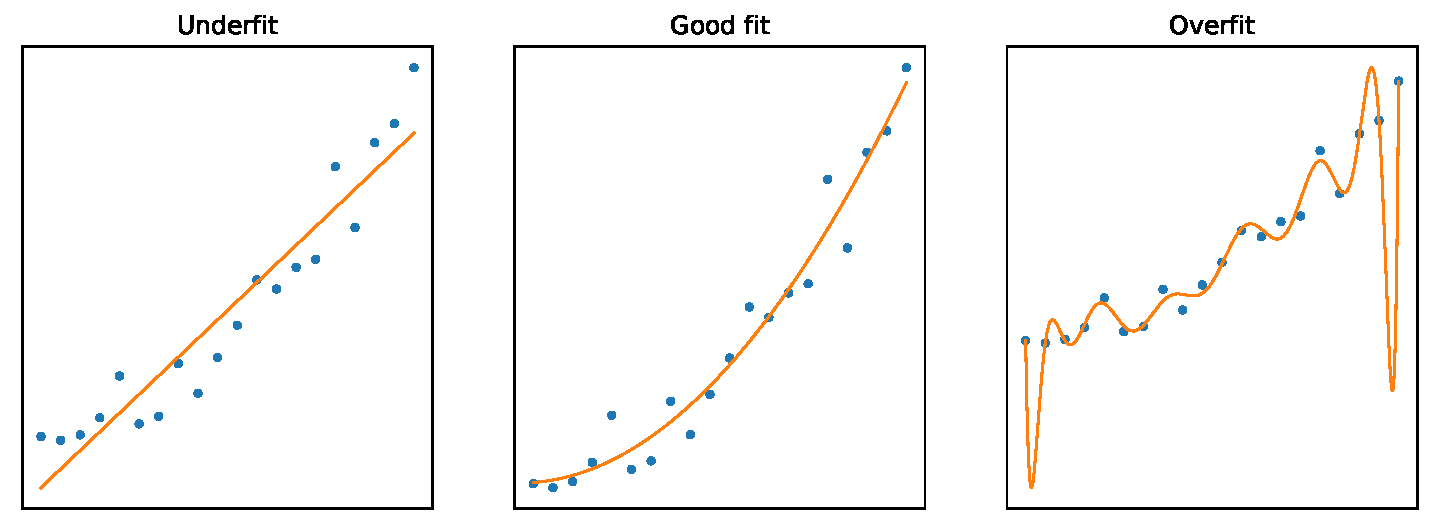
\includegraphics[width=0.8\textwidth]{chapters/NeuralNets/figures/fitting.pdf}
    \fonte{From the author (2021)}
    \label{fig:fitting}
\end{figure}
When the dataset is insufficient or the learning algorithm is not capable enough, the final model will only partially represent the data, but will not be able to capture all the details of the representation; this is called \textit{Underfitting}, the model was not able to fully represent the structure of the problem. In the other hand, the algorithm can also go to the opposite extreme and learn the dataset too well, this means that it will pick up particularities of the training data that don't generalize to the whole input distribution; this is called \textit{Overfitting} and it is facilitated by small datasets that don't represent much variety (noise in a sample has more influence in the signal to noise ratio of the whole dataset), or by networks that have too many degrees of freedom. \autoref{fig:fitting} visually represents the different fits for a 1-dimensional case.

Overfitting is however so common that it is almost natural to expect it's appearance, it is one of the most prevalent problems in machine learning and there are many existing techniques to avoid it. The first step is to have a good quality dataset, data augmentation methods can be used to easily multiply the number of samples without much downsides. In the algorithmic side, next subsection will discuss regularization and how it can combat overfitting among other things.

\subsection{Regularization} \label{sub:regularization}
According to \cite[p. 117]{deepLearningBook2016}: ``\textit{Regularization is any modification we make to a learning algorithm that is intended to reduce its generalization error but not it's training error}''. This is a general definition that encompasses many different techniques for regularization, but for this document it will suffice to describe only dropout and the $\ell_1$ and $\ell_2$ norms.

\subsubsection{L1 and L2 norms}
Since one of the reasons overfitting happens is because the models are given a large number of free parameters to adjust to the dataset (worth mentioning again the 175 billion parameters present in GPT-3 \cite{gpt3_2020}), then a common way of reducing overfitting is to limit the choice of parameters by adding a penalization term $\Omega(\bm{\theta})$ to the loss function as shown in \autoref{eq:regularization_penalty} \cite[p. 226]{deepLearningBook2016}.
\begin{equation} \label{eq:regularization_penalty}
    \tilde{J}(\bm{X}, \bm{\theta}) = J(\bm{X}, \bm{\theta}) + \lambda\Omega(\bm{\theta})
\end{equation}

The \gls{lambda} term is a positive hyperparameter that determines how much the penalty is relevant to the overall loss. For $\ell_1$ and $\ell_2$ norms, $\Omega(\bm{\theta})$ will be the respective norm of the $\bm{\theta}$ parameters. The $\ell_2$ norm is the standard distance in euclidean space, so for this norm the penalty term is given by \autoref{eq:l2_norm}.
\begin{equation} \label{eq:l2_norm}
    \ell_2(\bm{\theta}) = \|\bm{\theta}\|_2 = \sqrt{\theta_0^2 + \theta_1^2 + \dots + \theta_n^2}
\end{equation}

For the $\ell_1$ norm, the value calculated is what is called the Manhattan distance or taxicab distance \cite[p. 102]{dataDrivenScience2019} and is calculated as shown is \autoref{eq:l1_norm}
\begin{equation} \label{eq:l1_norm}
    \ell_1(\bm{\theta}) = \|\bm{\theta}\|_1 =  |\theta_0| + |\theta_1| + \dots + |\theta_n|
\end{equation}

Both norms will penalize large parameter values and the modified loss function in \autoref{eq:regularization_penalty} will make gradient descent favor solutions that use smaller parameters. The \gls{lambda} hyperparameter then determines how much to favor these simpler solutions.

A simple explanation on why smaller values would reduce overfitting can be given by considering the case of fitting a polynomial to some data. Consider the overfitting case seen before in \autoref{fig:fitting}, fitting a polynomial to reduce the square error on that noisy data results in a reasonable good approximation around the data points, but the curve suddenly changes directions in the extremes because of the terms with the highest powers in the polynomial. To make the curve fit the noisy data, a least squares approach will usually produce very high coefficients to balance the higher powers, this reduces the error but will almost never produce the true behaviour behind the data. Penalizing high coefficients with regularization is a way to force the solution to assume simpler values.

This is in no way a rigorous argument for regularization, but it can be used to have an intuition. The goal of this section is just to introduce the concept, regularization is an active area of research and a lot of support for it is based on empirical evidence, there is no complete theory to explain how and why it works so well \cite[chap. 3]{NN&DL2015}.

One last thing to mention is the fact that $\ell_1$ norm promotes sparsity in the parameters, this means that this approach will usually find solutions where multiple parameters will equal zero, larger values of \gls{lambda} will promote more sparse models.

\subsubsection{Dropout}
Since the local minimum reached by a training process will depend on the starting values for the parameters, one common way to increase the accuracy of a model is create an ensemble of different networks trained in the same dataset but with different starting points and/or architectures \cite[Chapter 6]{NN&DL2015}. The model output can then be a combination of the outputs of the ensemble, the combination could be majority voting, an average between outputs, or any other sensible function. This gives better results because it is not expected that randomly initialized networks would make the same mistakes in all situations \cite[p. 253]{deepLearningBook2016}.

Dropout is a technique that can be interpreted as a way to approximate an exponentially large ensemble of networks while using a single network and without needing to train more models \cite{dropout2012}. The idea behind it is that during training, when feedforwarding the input through the network, some units should have a probability $p$ of being dropped from the calculation, that is, their activations are set to zero.

The idea of removing units during calculation may sound counter-intuitive, but like the $\ell$ norms it is a way of restricting the learning process so that the network can't build very complex connections. By removing random units in each iteration, the network must be able to learn to represent the data even if a great number of units are removed, it no longer can expect that a combination of units will be present when evaluating the result and so it cannot depend on complex inter-correlations between units \cite{dropout2012}.

By dropping different units, dropout effectively trains the ensemble of all sub-networks of the base network. Typical dropout rates are 20\% for the input layer and 50\% for hidden layers \cite[p. 255, 257]{deepLearningBook2016}.

\subsection{Optimizers} \label{sub:optimizers}
Gradient descent has the theoretical basis for convergence, but it has big problems for use in practice. The first problem is that the whole training set must be averaged when calculating the loss $J(\bm{\theta})$, even for small datasets this is quite restrictive, for larger datasets containing hundreds of thousands or millions of samples this can make each iteration take an immense amount of time. This type of approach is commonly called Batch Gradient Descent.

Another problem is that, even if calculating the gradient was very fast, the simple parameter update (recall \autoref{eq:gradient_descent}) can become very slow, specially later in training. The point in parameter space can reach a region in the loss surface where the curvature is minimal, making the gradients very small; the updates could also jump around a valley in the loss surface, never reaching the local minimum \cite{momentumWorks2017}.

For calculating the gradients faster there is the approach called \glsreset{SGD}\gls{SGD}. There are several different methods for better traversing the loss surface, these are called optimizers. For the purposes of this document only the Momentum, RMSProp, and \gls{Adam} optimizers will be briefly explained.

\subsubsection{Stochastic Gradient Descent}
Instead of calculating the gradient $\nabla_{\bm{\theta}} J$ for all inputs in the dataset, \gls{SGD} instead approximates this value by calculating it for a single sample on the input. This makes the updates much faster, but will cause the updates to fluctuate heavily because of the gross approximation; this however can be beneficial since it can make the updates jump to potentially better local minima and it has been shown that, for small learning rates, \gls{SGD} will also converge \cite{optimizers2016}.

Another way to approximate the gradient is by calculating it only for a mini-batch of the dataset, that is, a subset of $m$ samples of the data. This is called Mini-batch Gradient Descent but is also more commonly referred to as \gls{SGD} as well. Using mini-batches instead of a single sample gives more stable updates while still being very fast, the values for $m$ usually fall between $50$ and $256$ \cite{optimizers2016}, but lower values are also common.

Another advantage of the stochastic approach is that the noise in the gradient approximation has an added regularization effect \cite[p. 5]{practical_gradient_recomendations2012}.

\subsubsection{Momentum, RMSProp, and Adam}
\glsreset{Adam}
The simple parameter update (\autoref{eq:gradient_descent}) for Gradient Descent has some problems that make it difficult to converge in practice. Some of the problems mentioned by \textcite{optimizers2016} are: that it is hard to choose a good value for the learning rate; only using a single learning rate can be insufficient; the parameters can get stuck in difficult regions of the loss surface, especially saddle points.

Between the many different approaches to combat this, one of the most popular that is also recommended when training \acp{GAN} \cite[p. 20, 27]{nipsGAN2017} is the \gls{Adam} optimizer. This optimizer is essentially a combination of Momentum and RMSProp, two other very popular optimizers.

Momentum, as the name suggests, is a way to give some inertia to the gradient updates, accelerating in the consistent directions while dampening oscillations. This technique has a strong theoretical basis and can give a quadratic speedup on many functions \cite{momentumWorks2017}. Momentum changes the parameter updates by adding a velocity term controlled by a new hyperparameter $\beta$ as shown in the following equations.
\begin{gather} \label{eq:momentum}
    \bm{m}_{i} = \beta \bm{m}_{i-1} + \nabla_{\bm{\theta}} J(\bm{\theta}_{i-1}) \\
    %
    \bm{\theta}_{i} = \bm{\theta}_{i-1} - \eta \bm{m}_{i}
\end{gather}

The RMSProp algorithm also tries to reinforce movement to the most relevant directions, it does this by keeping a exponentially moving average $v$ of the gradient accumulation \cite[303-304]{deepLearningBook2016}. It also introduces another $\beta$ hyperparameter and changes the updates as follows.
\begin{gather}
    \bm{v}_{i} = \beta \bm{v}_{i-1} + (1 - \beta)\nabla_{\bm{\theta}} J(\bm{\theta}_{i-1})^2 \\
    %
    \bm{\theta}_{i} = \bm{\theta}_{i-1} - \frac{\eta}{\sqrt{\bm{v}_{i} + \epsilon}} \nabla_{\bm{\theta}} J(\bm{\theta}_{i-1})
\end{gather}

Recall that although these equations are represented in vector form, all operation are performed element-wise. Finally for the \gls{Adam} algorithm, it can be seen as a combination of the two previous algorithms. It introduces two new hyperparameters $\beta_1$ and $\beta_2$ and the parameter updates work as follows \cite{adam2017}.
\begin{gather}
    \bm{m}_i = \beta_1 \bm{m}_{i-1} + (1 - \beta_1) \nabla_{\bm{\theta}} J(\bm{\theta}_{i-1}) \\[5pt]
    \bm{v}_i = \beta_2 \bm{v}_{i-1} + (1 - \beta_2) \nabla_{\bm{\theta}} J(\bm{\theta}_{i-1})^2 \\[5pt]
    \hat{\bm{m}_i} = \frac{\bm{m}_i}{1 - \beta_1^i} \\[5pt]
    \hat{\bm{v}_i} = \frac{\bm{v}_i}{1 - \beta_2^i} \\[5pt]
    \bm{\theta}_i = \bm{\theta}_{i-1} - \eta \frac{\hat{\bm{m}_i}}{\sqrt{\hat{\bm{v}_i} + \epsilon}}
\end{gather}

\textcite{adam2017} mentions that good default values for the hyperparameters are $\alpha = 0.001$, $\beta_1 = 0.9$, $\beta_2 = 0.999$ and $\epsilon = 10^{-8}$. The Tensorflow library \cite{tensorflow2015} follows this default, only changing $\epsilon$ to a order of magnitude higher, that is, $\epsilon = 10^{-7}$.

\subsection{Batch Normalization}
One important aspect in training neural networks is the distribution of the inputs for a layer. As mentioned in \autoref{subsub:sigmoid} about sigmoid, \textcite{efficientBackprop2012} showed that inputs that are not zero centered will have some bias effect on parameter updates, to avoid this the layer inputs should all be shifted to have a mean of zero; the authors also suggest to normalize all inputs in order to have the same covariance and, if possible, to have their values be uncorrelated. This should significantly speed up the learning process since the network will not have to adapt to a different distribution for every input.

Normalizing inputs is then an easy and effective way for better learning, therefore being a very commonly used technique that will also be used for the experiments proposed in this document.

However \textcite{batchnorm2015} note that for any layer in the network, the normalization idea for it's inputs also applies; that is, any hidden layer feeding it's output to the next layer can be considered as an input layer for a sub-network consisting of all the subsequent layers. Therefore, the same advantages for normalized inputs would be beneficial by normalizing hidden layer outputs.

Looking from the training perspective, each training iteration updates all parameters at the same time, but the gradient change in a layer gives the best change considering that all other layers remain constant \cite[p.313-314]{deepLearningBook2016}. In reality, changing the parameters of the previous layers will affect the distribution of inputs for the current layer, this constant change to the inputs of a layer resulting from changes to previous layers is what \textcite{batchnorm2015} call \textit{internal covariate shift}.

To address these issues \textcite{batchnorm2015} proposed a technique known as \gls{BN}, this method can be applied to any hidden layer and it consists of normalizing the layer inputs by the mean and variance of all the inputs in the current mini-batch. So, for a mini-batch $\mathcal{B}$ of size $m$ and inputs $(\bm{x}_1, \dots, \bm{x}_m)$, the normalized inputs $\hat{\bm{x}}_i$ are calculated using the mean $\bm{\mu}_{\mathcal{B}}$ and variance $\bm{\sigma}_{\mathcal{B}}$ of the batch. Equations \ref{eq:batch_mean}, \ref{eq:batch_variance}, and \ref{eq:batch_normalized_input} show how the mean, variance, and normalized inputs are calculated.
\begin{gather}
    \bm{\mu}_{\mathcal{B}} = \frac{1}{m}
    \sum_{i=1}^{m}{\bm{x}_i} \label{eq:batch_mean} \\[5pt]
    %
    \bm{\sigma_}{\mathcal{B}}^2 = \frac{1}{m}
    \sum_{i=1}^{m}{ \left( \bm{x}_i - \bm{\mu}_{\mathcal{B}} \right)^2 } \label{eq:batch_variance} \\[5pt]
    %
    \hat{\bm{x}}_i = \frac{ \bm{x}_i - \bm{\mu}_{\mathcal{B}} }
    { \sqrt{\bm{\sigma}_{\mathcal{B}}^2 + \epsilon} } \label{eq:batch_normalized_input}
\end{gather}

Note that these operations are applied element-wise for each component of the vectors, and again $\epsilon$ is used for numerical stability.

These operations result in the vectors $\hat{\bm{x}}_i$ having a mean of $0$ and variance of $1$ for each of their dimensions. However, by limiting the distribution to only these values also limits the representation power of the network \cite{batchnorm2015}, so the last step is to scale each one of the normalized activations by two new learnable parameters, $\gamma$ and $\beta$, unique for each activation, to obtain the transformed input $\bm{y}_i$ that can have any mean and variance. \autoref{eq:batch_transformed_input} shows how to scale the dimension $k$ of the normalized input $i$.
\begin{equation} \label{eq:batch_transformed_input}
    y_i^{(k)} = \gamma^{(k)} x_i^{(k)} + \beta^{(k)}
\end{equation}

This method has proven to be very powerful, with the original paper being able to reach the same accuracy as the, at the time state of the art image classification model, in 14 times less training iterations \cite{batchnorm2015}. The authors also cite a regularization effect of \gls{BN} that can reduce the need for other techniques like dropout.

When the authors originally proposed this method, they recommended applying the batch normalization operation directly to the weighted inputs of the network and only after apply the activation to the normalized values. However, since then \textcite{CaffeNetBench2017} empirically showed that applying \gls{BN} after the activation produces better results.

\subsection{Vanishing Gradients} \label{sub:vanishing_gradients}
Recall that for Equations \ref{eq:delta_last_layer} and \ref{eq:delta_hidden_layer} the $\delta$ term used to calculate the gradients, was directly dependent on the derivative of the activation function with relation to the weighted inputs $f'(\bm{z}^{(l)})$. Also note that the gradients are backpropagated through the network, which means that the $\delta$ values in a hidden layer are calculated from the $\delta$ in the next layer.

Consider now the case for a sigmoid or \gls{tanh} activation function which is applied to an weighted input far from zero, the activation in this case will be very close to the maximum or minimum value that the function can produce. When a unit outputs this kind of value it is said that it saturated, any slight deviation in the weighted input will barely have any difference in the activation value, in other words the derivative of the activation is close to zero.

Combining the points made in the last paragraphs it is possible to recognize a problem, when a unit saturates it's gradient will be very small since the derivative of the activation is close to zero. Even worse than that is the fact that this small gradient will be backpropagated through the network, reducing the gradients of all previous layers. When many units saturate, this effect can compound, making the gradients for deeper layers very small and greatly reducing the training speed; this is the problem known as the \textit{Vanishing Gradients} problem.

One alternate case is when the gradients are high and compound to make the gradients in deeper layers become very high, making the steps too large and not converging to any local minima. This is called the \textit{Exploding Gradients} problem.

Both situations are undesirable and are specially worrying when trying to train very deep neural networks. Ideally the gradients should all be close to $1$ to make training consistent, but for saturating activation functions like sigmoid, there will usually be vanishing gradients \cite{NN&DL2015}. That is one of the main reasons to use non-saturating activation functions like \gls{ReLU} in the hidden layers of the network. Other common ways to combat this problem is to carefully initialize the network parameters and use small learning rates \cite{batchnorm2015}, these authors also suggest that \gls{BN} can be used on saturating units since it can reduce the chance that the input of the units will fall to the saturating regions.
